\section{Introduction}

Whereas numerous works have been developed on example-based texture
synthesis (ETS)~\cite{Heeger:95, Portilla:2000:IJCV,
  Efros:sig2001,Kwatra:2003, Lefebvre:2005:sig, Ma:2011,
  dai:facade:iccv13} and are able to generate a variety of textures
from small examples, no one has systematically studied the
synthesizability of a texture example -- how well its underlying
visual patterns can be re-synthesized by learning only from this
example. This is contrary to other image properties that have been
studied, such as image quality~\cite{image:quality},
memorability~\cite{image:memorability},
interestingness~\cite{image:interestingness}. In this paper, we are
interested in learning image synthesizability and verifing its
usefulness in multiple applications.

Texture mapping adds detailed appearance of surface by projecting a
digitized texture image onto a surface. Although the technique itself
is straightforward, acquiring the texture images of desired size and
shape is not trival. The problem is pronounced as current large-scale
graphics applications require massive amounts of such textures. While
ETS has been proven a powerful tool to generate them~\cite{WLKT09},
providing massive amounts of `synthesizable' examples is not a trival
task. ETS systems expect a square image representing a flat,
outlier-free texture surface. 
% , and assume that the single example
% carries sufficient information about the underlying texture patterns
% for re-synthesis. 
The requirement is hard to enforce for large-scale applications:
texture examples obtained from image searching engine (by keywords)
possibly contain outliers, cluttered backgrounds, distorted texture
surfaces, or even objects of other categories. Thus, there is a clear
need to predict the synthesizability of these images in order to
filter out the unsynthesizable ones. Image synthesizability can also
be used to guide an image trimmimg process to make retrieved texture
examples more synthesizable. Also, there is no database with
annotations of the synthesizability of each image.
Fig.~\ref{fig:synlity} shows the synthesizability of some image
examples detected by our system and Fig.~\ref{fig:roi} shows the most
synthesizable regions detected by our system.

 
\begin{figure} [!t]
  \centering
   $ \begin{array}{cccc}
\hspace{-1.5mm}
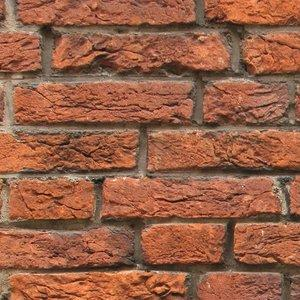
\includegraphics[width=0.33\linewidth]{./figs/1/1.jpg} & 
\hspace{-3mm}
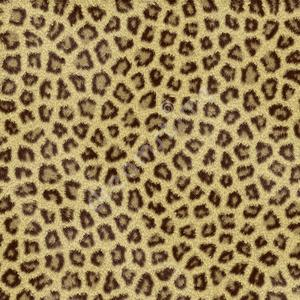
\includegraphics[width=0.33\linewidth]{./figs/1/43.jpg}&
\hspace{-3mm}
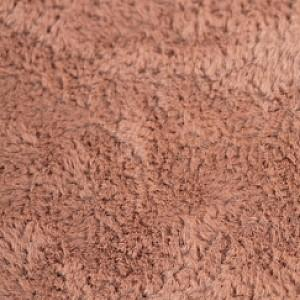
\includegraphics[width=0.33\linewidth]{./figs/1/60.jpg} \\
\scriptsize{\text{\textcolor{red}{0.98}}} & \scriptsize{\text{\textcolor{red}{0.90}}} & \scriptsize{\text{\textcolor{red}{0.85}}} \\
% \hspace{-3mm}
% 455 0.56 feature.jpg 0.66   512 0.41   96 0.44 cliff3.jpg 0.40 
\hspace{-1.5mm}
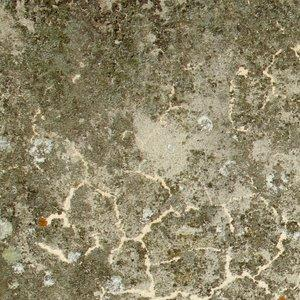
\includegraphics[width=0.33\linewidth]{./figs/1/55.jpg} & 
\hspace{-3mm}
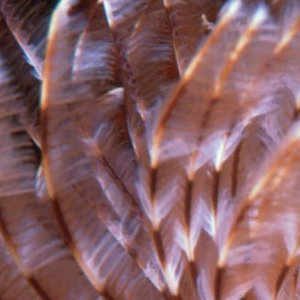
\includegraphics[width=0.33\linewidth]{./figs/1/feather.jpg}&
\hspace{-3mm}
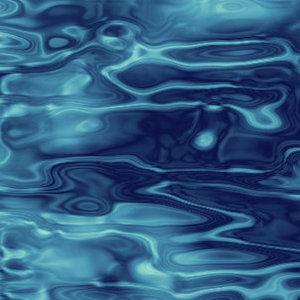
\includegraphics[width=0.33\linewidth]{./figs/1/40ee.jpg} \\
\scriptsize{\text{\textcolor{red}{0.79}}} & \scriptsize{\text{\textcolor{red}{0.66}}} & \scriptsize{\text{\textcolor{red}{0.56}}} \\
\hspace{-1.5mm}
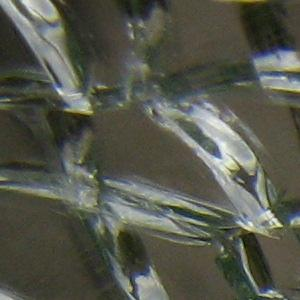
\includegraphics[width=0.33\linewidth]{./figs/1/96.jpg} & 
\hspace{-3mm}
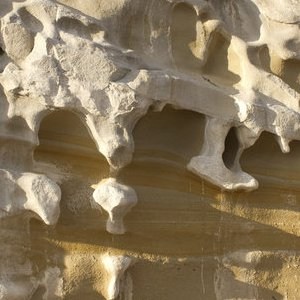
\includegraphics[width=0.33\linewidth]{./figs/1/cliff3.jpg}&
\hspace{-3mm}

\includegraphics[width=0.33\linewidth]{./figs/1/512.jpg} \\
\scriptsize{\text{\textcolor{blue}{0.44}}} & \scriptsize{\text{\textcolor{blue}{0.42}}} & \scriptsize{\text{\textcolor{blue}{0.36}}} \\
\hspace{-1.5mm}
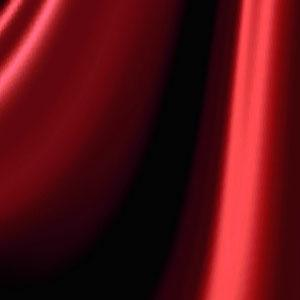
\includegraphics[width=0.33\linewidth]{./figs/1/427.jpg} & 
\hspace{-3mm}
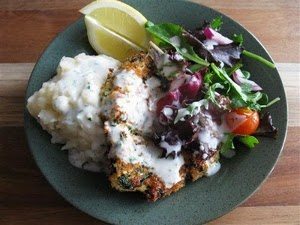
\includegraphics[width=0.33\linewidth, height=27.5mm]{./figs/1/faith4.jpg}&
\hspace{-3mm}
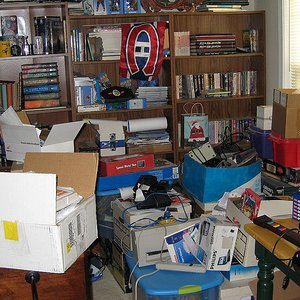
\includegraphics[width=0.33\linewidth]{./figs/1/shelf.jpg} \\
\scriptsize{\text{\textcolor{blue}{0.28}}} & \scriptsize{\text{\textcolor{blue}{0.25}}} & \scriptsize{\text{\textcolor{blue}{0.13}}} \\
% \hspace{-3mm}
% 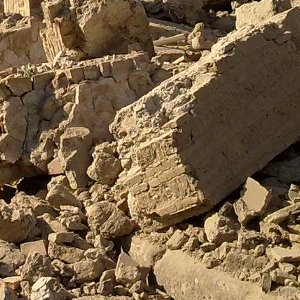
\includegraphics[width=0.25\linewidth]{./figs/1/wall.jpg} \\
\end{array}$
\caption{Synthesizability (Synlity) of texture examples detected by
  our system. All images are of $300\times 300$ pixels.}
  \label{fig:synlity}
\end{figure}


\begin{figure} [!t]
  \centering
   $ \begin{array}{cccc}
\hspace{-1.5mm}
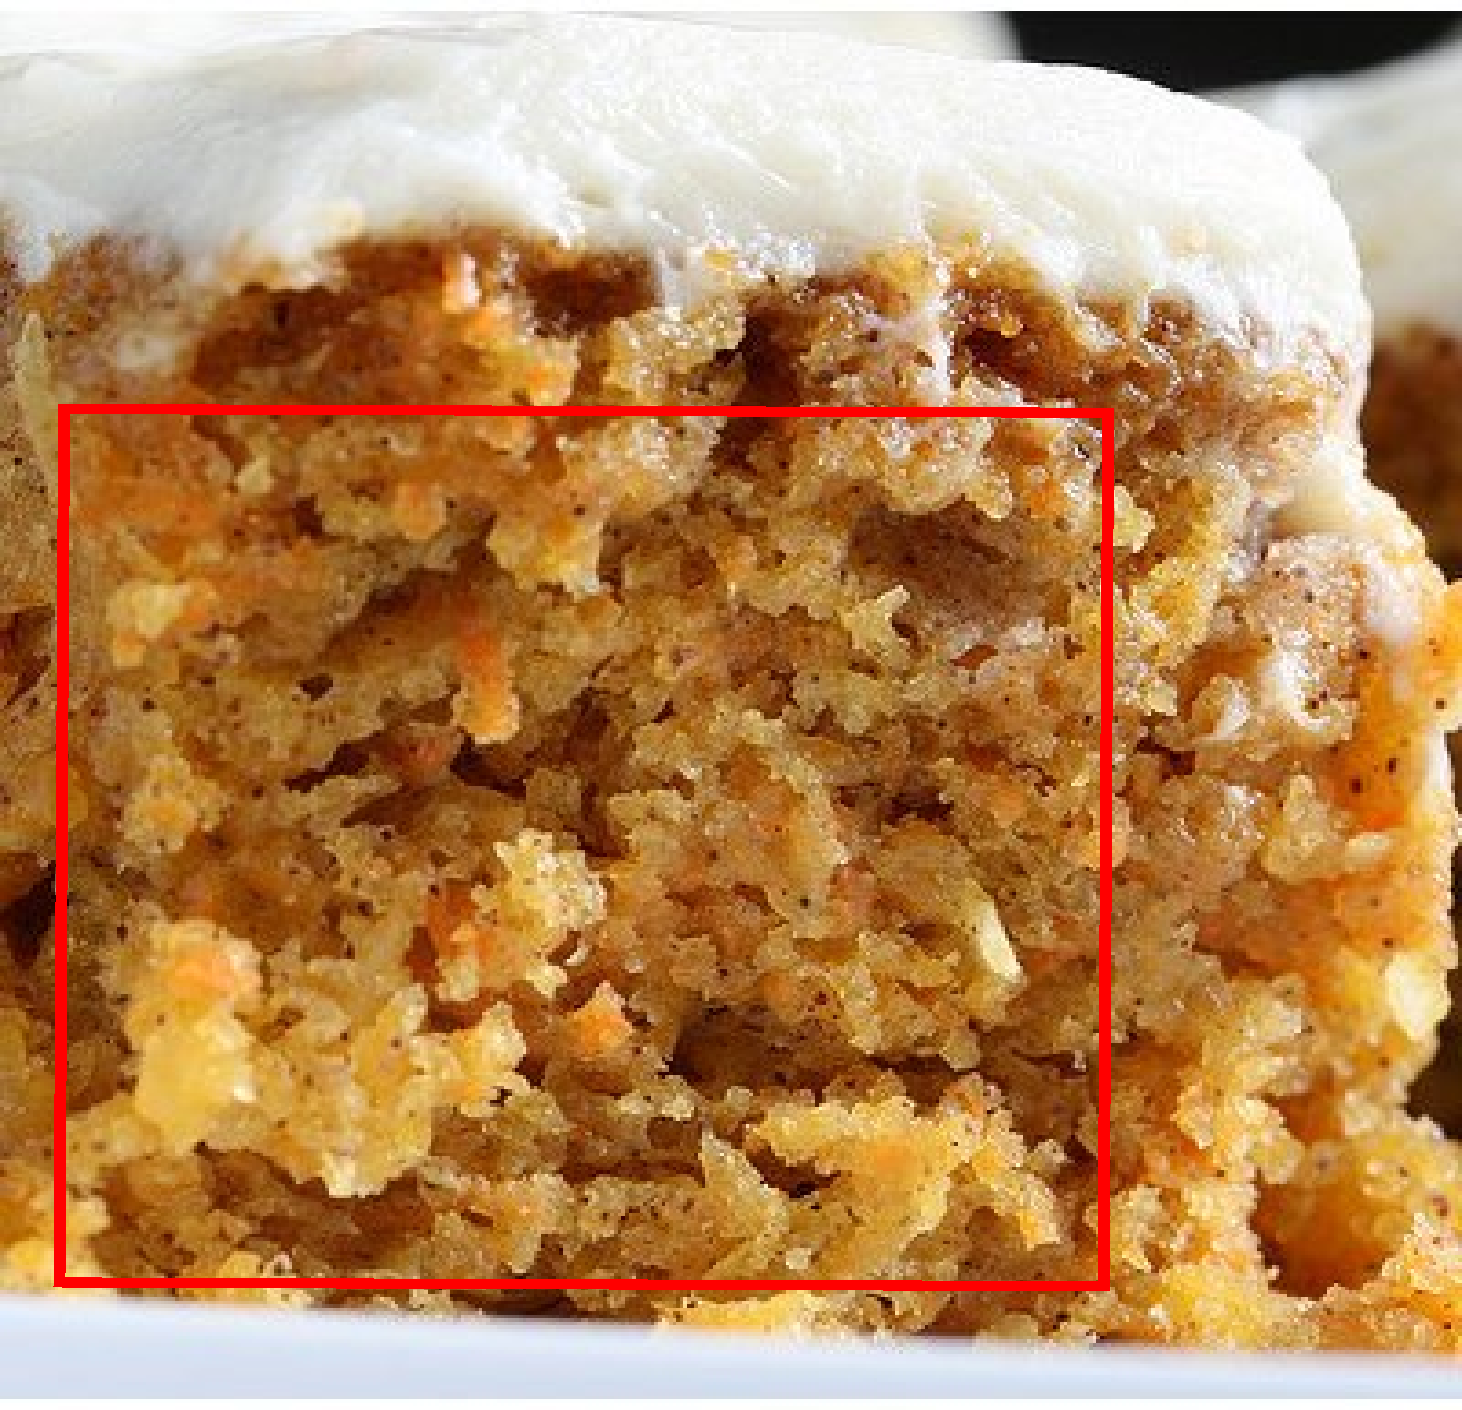
\includegraphics[width=0.48\linewidth, height=35mm]{./figs/2/2.pdf} & 
\hspace{-3mm}
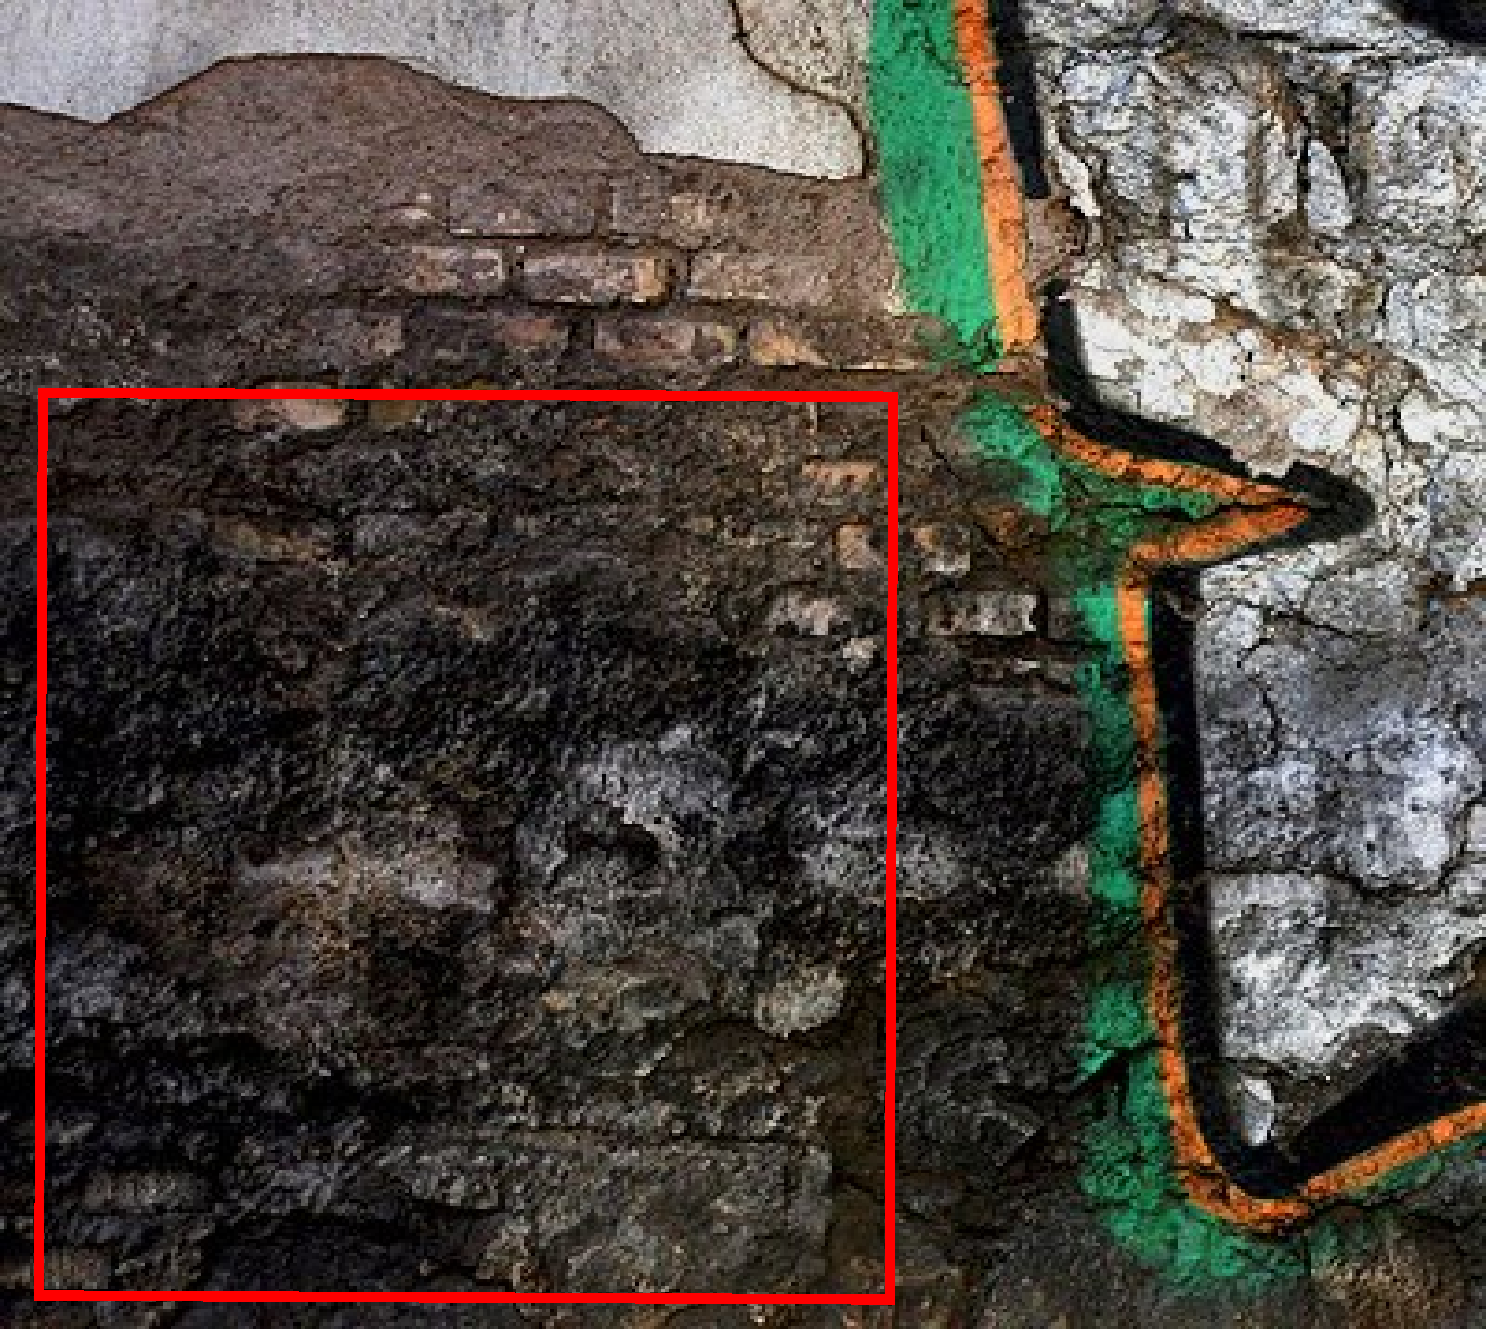
\includegraphics[width=0.48\linewidth, height=35mm]{./figs/2/3.pdf} \\
\scriptsize{\text{r-synlity:\textcolor{red}{0.92} \hspace{1mm} i-synlity:0.40}} & 
\scriptsize{\text{r-synlity:\textcolor{red}{0.67}, \hspace{1mm} i-synlity:0.50}}  \\
\end{array}$
\caption{The most synthesizable region detected by our system. 
Synthesizability of detected regions (r-synlity) and the whole images (i-synlity) are shown. }
  \label{fig:roi}
\end{figure}

In order to learn image synthesizability and evaluate its performance,
a fairly large texture database containing $32,000$ texture images is
constructed, and annotated according to the synthesizability of each
image.  We characterize image synthesizability as the `goodness' of
synthesized textures. A series of features are employed and designed
to computationally capture image synthesizability. Multiple learning
methods are used to learn it from the collection of data. Experimental
result show that image synthesizability is predictable by learning
from a large collection of data. We also show in experiments that
image synthesizability is a general image property and is helpful for
image recognition as well.

Our main contribution are: (1) learn the image property
synthesizability methodologically; (2) design several features for
texture analysis (esp. Repetitiveness, Irregularity); (3) collect a
fairly large texture dataset and annotate it in terms of
synthesizability; (4) verify the usefullness of synthesizability in
multiple vision applications.



